%\documentclass[oneside, final, 12pt]{extreport}
\documentclass[12pt,fleqn]{article}

\usepackage{amsmath, amsthm, amssymb} %math expressions, theoreme/lemma, math symbols
\usepackage{mathtext} %russian letters in formulas

% fonts and lang
%\usepackage[T1,TS1,T2A]{fontenc}
\usepackage{cmap}
\usepackage[T1, T2A]{fontenc}
\usepackage[utf8]{inputenc}
\usepackage[english, russian]{babel}

% formatting
% \usepackage{geometry} %customize page layout
% \geometry{left = 3cm}
% \geometry{right = 1cm}
% \geometry{top = 1.5cm}
% \geometry{bottom = 2cm}

\usepackage{setspace} %set space between lines
\usepackage{indentfirst} %indent first pagearagraph after section header

\usepackage{tocloft} %control table of contents, figures

\usepackage{graphicx}

\usepackage{hhline}

\usepackage{caption}

\usepackage{subcaption}

\usepackage[shortlabels]{enumitem}
\setlist{nolistsep, itemsep=0.1cm, parsep=0pt, leftmargin=1.5cm}

\usepackage{multirow}

\usepackage{algorithm}
\usepackage{algpseudocode}

\textheight=23cm
\textwidth=16cm
\oddsidemargin=5mm % левое поле для нечётных страниц
\evensidemargin=-5mm % севое поле для чётных страниц
%\marginparwidth=36pt
\topmargin=-1cm % расстояние от верхней границы листа до заголовка
%\flushbottom % выстота тела всех страниц одинаковая 
\raggedbottom % позволяет несколько различаться высоте тел различных страниц
\tolerance 3000 % how much badness is allowable without error. 

\linespread{1.3} %1.5 spacing 

\parindent 1.27cm % Абзацный отступ

\sloppy             % текст редко залезает на правое поле
\clubpenalty = 10000  % Запрещаем разрыв страницы после первой строки абзаца
\widowpenalty = 10000 % Запрещаем разрыв страницы после предпоследней строки абзаца
% \global\hyphenpenalty = 1000 % Частота переносов


%Разработка метода прогнозирования слабой масштабируемости суперкомпьютерных приложений

\begin{document}

	\begin{titlepage}
	\begin{center}
	    Московский государственный университет имени М.В.Ломоносова

	    \bigskip
	    
\includegraphics[width=50mm]{./images/MSU}

	    \bigskip
	    Факультет Вычислительной Математики и Кибернетики\\
	    Кафедра Суперкомпьютеров и Квантовой Информатики\\[10mm]

	    \textsf{\large\bfseries
	        ВЫПУСКНАЯ КВАЛИФИКАЦИОННАЯ РАБОТА\\[10mm]
	        <<Разработка метода прогнозирования слабой масштабируемости суперкомпьютерных приложений>>
	    }\\[10mm]

	    \begin{flushright}
	        \parbox{0.5\textwidth}{
	            Выполнил:\\
	            студент 4 курса 423 группы\\
	            \emph{Мокров Кирилл Сергеевич}\\[5mm]
	            Научный руководитель:\\
	            к.ф-м.н., ведущий научный сотрудник НИВЦ МГУ\\
	            \emph{Антонов Александр Сергеевич}
	        }
	    \end{flushright}

	    \vspace{\fill}
	    Москва, 2020
	\end{center}
\end{titlepage}

\clearpage
%\newpage

	\tableofcontents
	\thispagestyle{empty}
	\clearpage
	\setcounter{page}{3}

	\section{Введение}
	Без параллельных технологий сейчас невозможно обойтись во многих прикладных областях науки: гидро- и аэро- динамике, квантовая химии, сейсмике, компьютерном моделировании лекарств, криптографии и многих других. Это связано с необходимостью обрабатывать большие объёмы данных и производить колоссальное количество вычислений. Что стимулирует создание больших суперкомпьютерных центров, развитие технологий конструирования аппаратных комплектующих, разработку новых методик и алгоритмов.

	Если используемые пакеты прикладных программ и научные приложения будут плохо написаны, выбранный алгоритм слабо параллелизуем или неоптимально реализован в коде, то они не смогут в полной мере использовать вычислительные ресурсы, предоставляемые высокопроизводительным центром. Если рассмотреть результаты запусков бенчмарков HPL и HPCG на суперкомпьютерах из рейтинга TOP500 \cite{top500}, то окажется, что для HPL среднее отношение реальной и пиковой производительностей около 63.5\%, для HPCG этот показатель сильно ниже - около 1.5\%(результаты тестирования HPCG предоставлены только для 70 суперкомпьютеров). Данные бенчмарки - это сверх оптимизированные приложения, написанные в тесном сотрудничестве математиками и программистами, лишь малая часть параллельных программ имеют схожую степень параллелизуемости. В статье \cite{Perf_low} приводятся данные с достигаемой производительностью на реальных научных приложениях, моделирование распространения сейсмических волн, высокотемпературной плазмы, термоядерного синтеза, на суперкомпьютере Blue Water из Университета Иллинойса, по всем приложениям производительность не превышает 20\% от пиковой.
	% фундаментальные ограничения, как закон Амдала и закон Густавсона — Барсиса,

	Существует множество характеристик работы параллельных программ, например, время её выполнения, ускорение и эффективность, производительность, количество обращений в память и кэш-промахов. Все они имеют динамическую сущность, то есть могут изменяться от запуска к запуску, зависят от параметров запуска программы и машины, на которой она выполняется, поэтому будем называть их динамическими характеристиками параллельной программы.

	Чтобы понять свойства параллельных программ и причины найденных в них особенностей, нужно рассматривать все доступные динамические характеристики на всём пространстве параметров запуска. Эта задача напрямую связана с понятием "<масштабируемость">, свойством параллельной программы, характеризующим зависимость изменения всей совокупности динамических характеристик работы этой программы от множества параметров её запуска \cite{scalability_def}.

	Здесь и далее обозначим: \(p\) - количество процессов, на которых запущено приложение; \(N\) - размера задачи; \(T_A(N)\) - сложность алгоритма \(А\) для значения \(N\) размера входа. \(T_A(N) = \max_{||y|| = N} C^T_A(y)\), где \(C^T_A(y)\) сложность алгоритма \(А\) для входа \(y\) \cite{COMPLEXITY}. Сложность алгоритма следует понимать, как последовательную сложность, то есть, как число операций, которое нужно выполнить при последовательном выполнении алгоритма.

	Во время исследования масштабируемости приложения необходимо указывать, на какой области изменения значений параметров проведены запуски. По выбору параметров запуска, которые будут изменяться, масштабируемость согласно \cite{scaling_types} можно разделить на три основных типа:
	\begin{itemize}
		\item Сильная масштабируемость (strong scaling) - зависимость динамических характеристик от количества процессов \(p\) при фиксированной вычислительной сложности задачи \((T_A(N) = const \Rightarrow N = const)\).
		\item Слабая масштабируемость (weak scaling) - зависимость динамических характеристик от количества процессов \(p\) при фиксированной вычислительной сложности задачи в пересчете на один узел \((T_A(N)\:/\:p = const)\)
		\item Масштабируемость вширь (wide scaling) - зависимость динамических характеристик от размера задачи при фиксированном количестве процессов \((p = const)\)
	\end{itemize}

	Масштабируемость - ключевое понятие в вопросах исследования свойств параллельных программ, поэтому крайне важно учитывать её на всех этапах разработки программного обеспечения. Однако не всегда возможно получить в распоряжение большое количество узлов, чтобы увидеть характер изменения различных динамических характеристик приложения с ростом числа используемых ресурсов системы, при увеличении размера задачи, или ожидание этого может занять непозволительно много времени, например, авторы статьи \cite{log_main} утверждают, что в худшем случае время ожидания выделения необходимого количества узлов растёт экспоненциально с ростом количества запрашиваемых ресурсов. Но ведь именно возможность решать задачи больших размеров за разумное время, используя большое количество узлов, является главным преимуществом суперкомпьютерных систем, поэтому необходимо, чтобы приложение было хорошо масштабируемо. Обычно пользователь может выполнить задачу на небольшой конфигурации быстрее, чем запустить на большом количестве узлов. Исходя из этого, актуальна задача прогнозирования масштабируемости приложения на большие конфигурации вычислительной системы, основываясь только на данных, полученных из множественных запусков на малых конфигурациях. В данной работе предлагается механизм решения поставленной задачи в условиях слабой масштабируемости суперкомпьютерных приложений.
\clearpage
%\newpage
	%Разработка метода прогнозирования слабой масштабируемости суперкомпьютерных приложений
\section{Постановка задачи}
	Целью данной работы является разработка метода прогнозирования слабой масштабируемости суперкомпьютерных приложений. На разрабатываемый метод накладываются условия универсальности, то есть для своей работы он не должен использовать информацию о коде, алгоритме и системе, на которой производятся запуски.

	Для достижения данной цели требуется решить следующие задачи:
	\begin{itemize}
		\item Разработать метод, предсказывающий слабую масштабируемость суперкомпьютерных приложений на основе экспериментальных данных.
		\item Проверить применимость метода на различных приложениях, собрав экспериментальную базу и оценив точность предсказаний.
	\end{itemize}


\clearpage
% \newpage
%На счёт же третьей постановки - если мы ставим задачу разработки программного средства, то это средство нужно будет предъявить, и к нему будут предъявлять все обычные требования как к программному средству по оформлению, документированию и т.д., об этом тогда тоже не забудьте позаботиться.
	\section{Обзор существующих подходов к предсказанию масштабируемости}
%как свойства параллельной программы, характеризующего зависимость изменения всей совокупности динамических характеристик работы этой программы от множества параметров её запуска
	Когда говорят о предсказании масштабируемости, то рассматривают не всю совокупность динамических характеристик работы программы, а её часть. Большинство исследований направлены на предсказание времени исполнения программы в зависимости от параметров её запуска. Также существуют работы, рассматривающие предсказание производительности, ускорения, эффективности и энергопотребления. Однако этими характеристиками всё не ограничивается, так, например, в исследовании \cite{efficiency_prediction} авторы строят модель, предсказывающую несколько не совсем стандартных характеристик параллельной программы: первая отражает потенциальную потерю эффективности, вызванную различным временем вычислений разных процессов, вторая - неэффективность, вызванную зависимостями в коде, а третья - потерю производительности, вызванную передачей данных.
	%Ими также как и в \#LINK\# исследуется возможность предсказания данных характеристик приложения на больших конфигурациях, построенного на основе запусков на малых конфигурациях. \#мб результаты убрать\# Модель тестируется с помощью приложений из CORAL(HACC, Nekbone, AMG2013) и приложения AVBP. Запуски HACC и Nekbone проводятся в условиях сильной масштабируемости, а AMG2013 и AVBP - в условиях слабой. Получившиеся значения относительных ошибок варьируются от 0.01\% до 27.19\%.

	%Существует большое число работ направленных на исследование и предсказание масштабируемости приложений на суперкомпьютерах,
	Большинство работ направлено на исследование и предсказание масштабируемости приложений на суперкомпьютерах, но встречаются и такие, которые используют для запуска параллельных приложений отдельные узлы, небольшие вычислительные системы, грид-системы, платформы для облачных вычислений.

	Все исследования можно разделить на две группы: первая объединяется в себе те труды, которые ставят перед собой цель, используя запуски на малых конфигурациях, экстраполировать их результаты на большие; вторая же состоит из тех работ, которые, основываясь на результатах запусков, равномерно распределённых по пространству параметров, пытаются интерполировать их на всё пространство параметров.

	Наиболее распространёнными для предсказания масштабируемости являются подходы, использующие аппарат линейной регрессии, методы машинного обучения, а именно нейронные сети, симуляцию исполнения программы и коллаборативную фильтрацию. Все они будут рассмотрены в следующей части этой главы.

	\subsection{Линейная регрессия}
		В статье \cite{log_main} предложены 3 техники предсказания масштабируемости параллельных программ, в основе которых лежит подбор коэффициентов линейной регрессии. Эти техники используют набор запусков приложений на небольшом количестве процессов с разными входными парамерами, чтобы предсказать производительность на большом количестве процессов. Первая техника является идейно самой простой: результаты тестовых запусков используются для подбора коэффициентов регрессии, а затем с помощью построенной модели результаты экстраполируются на конфигурации большого размера. Вторая и третья техники являются усовершенствованиями первой, они обе рассматривают время вычислений и время коммуникаций отдельно. Отличия в том, что вторая техника основывается на временах вычислений и коммуникаций, полученных от каждого из процессов, выбирая максимальный по времени вычислений процесс и используя его же время коммуникаций, а третья техника основывается на определении времени коммуникаций и вычислений на критическом пути, самой длинной последовательности выполнения программы без блокировок.

		В статье рассматривается сильная масштабируемость, где это возможно, то есть, где задача помещается в память при выполнении на малом количестве процессов, или гибрид сильной и слабой масштабируемостей. Строятся предсказания времени выполнения программы на большом количестве процессов, используя несколько запусков той же программы на меньшем количестве. Для оценки качества предсказаний используется относительная ошибка. Из-за этого необходимо применять приближение в логарифмическом масштабе, а с учётом того, что авторами выбрана линейная регрессионная модель, формулу предиктора можно записать в виде:
		\[
		\log_2{(T)} = \sum_{i=1}^{n}{\beta_i\log_2{(x_i)}} + g(p) + error
		\]
		Где для выражения, объясняющего вклад количества используемых процессов выбирается либо линейное, либо квадратичное представление:
		\[
		g(p) = \gamma_0 + \gamma_1\log_2(p) + [\gamma_2log_2^2(p)]
		\]
		Несмотря на наличие логарифмов, статистически это всё ещё линейная модель, поскольку она линейна относительно неизвестных параметров.


		% \(p\) процессах, используя несколько запусков той же программы на \(q\) процессах, где \(q \in \{2,\ldots, p_0\},\,p_0 < p\), для произвольного \(p\). Предиктор реального времени исполнения \(T\) представляет собой функцию зависящую от входных параметров \((x_1, x_2, \ldots, x_n)\) и количества используемых процессов \(q\):
		% \begin{equation}\label{lin_formula}
		% \hat{T} = F(x_1, x_2, \ldots, x_n, q)
		% \end{equation}
		% Для оценки качества предсказаний используется относительная ошибка, вычисляемая по формуле:
		% \begin{equation}
		% E = \frac{|T - \hat{T}|}{T}
		% \end{equation}
		% Из-за того что используется относительная ошибка для оценки модели, \(F\) должная приближать \(T\) в логарифмическом масштабе, а с учётом того, что авторами используется линейная модель, формула \ref{lin_formula} преобразуется в
		% \begin{equation}
		% \log_2{(T)} = \sum_{i=1}^{n}{\beta_i\log_2{(x_i)}} + g(q) + error
		% \end{equation}
		% , где для выражения, объясняющего вклад количества используемых процессов используется либо линейное, либо квадратичное выражение:
		% \begin{equation}
		% g(q) = \gamma_0 + \gamma_1\log_2(q) + [\gamma_2log_2^2(q)]
		% \end{equation}
		% Несмотря на наличие логарифмов, статистически это всё ещё линейная модель, поскольку она линейна относительно неизвестных параметров.

		Для различных приложений медианная ошибка предсказаний изменяется от 1\% до 92\% в случае с первой техникой и от 7\% до 67\% для второй и третьей техник.

		Построенная модель обладает несколькими недостатками: не всегда возможно разделить время коммуникаций и вычислений, а чтобы это сделать, возможно, необходимо обладать знаниями об исходном коде программы или быть способным его модифицировать, поэтому использование второй и третьей техник не всегда представляется возможным. Также неясно, какой вид для функции \(g(q)\) следует выбрать. Дополнительно авторами метода прогнозирования предполагалось, что исследуемые задачи обладают хорошей вычислительной сбалансированностью, но далеко не все параллельные приложения отвечают этому предположению.

		%%%%%%%%%%%%%%%%%%%%%%%%%%%%%%%%%%%%%%%%%%%%%%%%%%%%%%%%%%%%%%%%%%%%%%%%%%%%%%%%%%%
		Такой же подход, использование линейной регрессии и логарифмической шкалы, применяется в работе \cite{focused_regression}. В ней авторы ставят перед собой задачу разработать модель, позволяющую находить конфигурации запуска так, чтобы они находились на кривой постоянного времени работы приложения, если в качестве пространства параметров конфигураций рассматривать размер задачи и количество процессов, на которых будет запущено приложение. Для построения модели используется информация о том, есть ли связь между параметрами запуска приложения, специфицируется ли при запуске процессорная сетка, позволяющая контролировать распределение данных, и набор запусков приложения на небольшим количестве процессов. Экспериментальная проверка построенной модели на семи суперкомпьютерных приложениях позволила предсказать неизвестные значения параметров так, что медианная ошибка предсказаний получилась меньше 13\%.

		%%%%%%%%%%%%%%%%%%%%%%%%%%%%%%%%%%%%%%%%%%%%%%%%%%%%%%%%%%%%%%%%%%%%%%%%%%%%%%%%%%%%%%%%%%%%%%%%%%%%%%%%%%%
		Подход, предложенный в \cite{analytic_func}, отличается от всех остальных прежде всего тем, что строятся не просто предсказания значений той или иной динамической характеристики параллельной программы, а предлагается функция, описывающая изменение этой характеристики и зависящая от параметров запуска. Такой подход находит своё применение, когда необходимо оценить асимптотику поведения динамических характеристик, но построение точной, аналитической модели является затруднительной задачей.
			
		На первом этапе работы собирается такая информация, как время исполнения, значения различных аппаратных (количество операций с числами с плавающей запятой) и программных (количество байт, которые MPI функции отправили и приняли) счётчиков производительности. Чтобы обеспечить статистически значимый набор данных о производительности, измерения для одних их тех же конфигураций запуска проводятся несколько раз. Собранные результаты запусков разделяются на две группы: в первой находятся запуски на небольших конфигурациях, на них основывается работа по подбору коэффициентов, во второй - запуски на конфигурациях большего размера, именно на них поведение приложений представляет наибольший интерес, использующиеся для оценки качества предсказаний модели. С помощью профайлера Scalasca в коде программы выделяются фрагменты, так называемые ядра, к которым можно отнести вызовы MPI функций и наиболее вычислительно интенсивные участи кода. Далее, используется регрессия для получения грубой модели производительности для каждого ядра. В качестве моделей рассматриваются выражения вида:
		\[
		f(p) = \sum \limits_{k=1}^{n} c_k \cdot p^{i_k} \cdot \log_2^{j_k}(p),\; i_k \in I,\; j_k \in J 
		\]
		Где \(I\) и \(J\) заданные заранее множества. Эти модели позднее проходят итеративный процесс уточнения, во время которого методами регрессионного анализа подбираются наиболее оптимальные значения \(c_k\) для всевозможных троек \(n,\;i_{k},\;j_{k}\), пока качество модели не достигнет точки насыщения. Если степень точности предсказаний недостаточна для получения действенной рекомендации, то исследуемые ядра могут быть дополнительно уточнены с помощью более подробного инструментария. Разработанный подход тестировался на приложениях SWEEP3D, MILC и предсказал асимптотики масштабируемости, в точности согласующиеся с ранее созданными точными моделями. Для приложения HOMME, масштабируемость которого раннее не исследовалась, и поэтому такой точной модели не было, предложенный авторами подход позволил обнаружить плохую масштабируемость одного из ядер, что затем полностью подтвердилось результатами проведённых экспериментов.

		Стоит отметить, что множества \(I\) и \(J\) задаются для каждого приложения по-своему, количество и значения элементов в них устанавливается исходя только из логических соображений, что не удовлетворяет требованиям универсальности, ведь результаты предсказаний напрямую зависят от человека, исследующего характеристики приложения и задающего эти множества.


	\subsection{Методы машинного обучения}
		Методы машинного обучения широко применяются для предсказания производительности параллельных приложений, так как построение точной аналитической модели приложения часто является очень затруднительным, а сами модели не способны уловить сложные аспекты взаимодействия между архитектурой суперкомпьютера и исследуемыми программами.

		В статье \cite{ML_SMG2000} трёхслойная полносвязная нейронная сеть прямого распространения с сигмоидой в качестве функции активации используется для предсказания времени работы приложения SMG2000. В процессе исследований авторы работы сталкиваются с двумя проблемами, из-за которых средняя ошибка предсказаний даже при использовании 10 тысяч запусков, равномерно распределённых по пространству параметров, в качестве обучающего множества, превосходит 15\%. Первая из проблем - это значительные шумы в результатах проведённых запусков, проявляющиеся в значительных падениях производительности. Они, например, могут возникать из-за работы операционной системы, использующей ресурсы вычислительного комплекса совместно с потоками исполнения приложения. В качестве способа преодоления этой проблемы авторы выбрали резервирование, как минимум, одного процесса на узле на нужды ОС. Вторая проблема является более серьёзной и не так просто преодолимой. Она заключается в ориентированности алгоритма подбора весов в нейронной сети на минимизацию среднего квадрата ошибки, в то время как качество предсказания оценивается по вычислениям относительных ошибок. Чтобы исправить это, применяются техники стратификации выборки с применением весов и беггинг для обучения ансамблей моделей и дальнейшего усреднения прогнозов. После осуществления вышеописанных изменений качество предсказаний значительно возрастает. Теперь при использовании 500 запусков средняя ошибка предсказаний не превышает 12\%, а при увеличении размера обучающей выборки в 5 раз, до 2500 запусков, авторы получают уменьшение средней ошибки до 6,5\%, что уже является достаточно высокой точностью.

		%%%%%%%%%%%%%%%%%%%%%%%%%%%%%%%%%%%%%%%%%%%%%%%%%%%%%%%%%%%%%%%%%%%%%%%%%%%%%%
		Применение нейронных сетей не ограниченно предсказаниями производительности на классических HPC системах, так технологии машинного обучения используют в \cite{ML_Grid} для предсказания времени работы научных приложений, состоящих из нескольких подзадач со сложными внутренними зависимостями, на Grid системах. Моделирование и предсказание времён выполнения таких приложений очень сложно из-за распределения и параллельного исполнения подзадач на столь разнородной системе и динамического поведения общих Grid ресурсов. Ошибка предсказаний рассматриваемой в работе трёхслойной нейронной сети с радиально-базисной функцией, в качестве функции активации, в среднем не превышает 12\%. Но стоит отметить, что для обучения потребовалось 10000 запусков рассматриваемых в статье приложений.

		%%%%%%%%%%%%%%%%%%%%%%%%%%%%%%%%%%%%%%%%%%%%%%%%%%%%%%%%%%%%%%%%%%%%%%%%%%%%%%%%%%%%
		Нейронную сеть такой же конфигурации, как в \cite{ML_SMG2000}, авторы \cite{ML_PROC_KERN} применют для предсказания наиболее оптимальных параметров запусков приложений на SMP системах. В качестве параметров рассматриваются количество процессоров и количество запрашиваемых ядер на одном процессоре. Поиск оптимальной конфигурации необходим, так как использование оптимальных параметров позволяет не только сократить время вычислений и, как следствие, увеличить производительность, но и уменьшить энергопотребление. Проведённые авторами эксперименты показали, что разработанная нейросеть позволяет достичь медианной ошибки предсказаний времени 7.5\% (для оценки используются показатели времени на предложенной нейросетью конфигурации и оптимальной конфигурации, найденной полным перебором).

	\subsection{Симуляция исполнения программы}
		Подход с использованием симуляции исполнения приложений является наиболее сложным в реализации. Он часто использует в своей работе информацию о структуре программы и о подробных технических характеристиках используемой системы, но, несмотря на это, подобные подходы встречаются.

		Так описанный в статье \cite{simulation_FASE} фреймворк FASE (The Fast and Accurate Simulation Environment) позволяет проводит симуляцию исполнений приложений на HPC системах. FASE предоставляет инструментарий для оценки производительности виртуально-прототипированных систем для своевременного и экономически эффективного определения идеальной конфигурации системы для конкретного набора приложений. Работа фреймворка состоит из двух этапов: сначала с помощью встроенных инструментов собирается некоторая характеристика рассматриваемого приложения, далее вводятся параметры системы (тип коммуникационной сети, сетевой протокол, информация об используемых процессорах, оперативной памяти), то есть создаётся некоторая модель системы. Если рассматривается производительность приложения на уже существующей системе и известны некоторые её характеристики, например, пропускная способность или среднее время задержки сети, то добавление этой информации на втором этапе позволит сделать предсказания FASE более точными. Полученные относительные ошибки предсказания времени выполнения приложения в большинстве случаев не превосходят 10\% для бенчмарка Sweep3D и 1\% для перемножения матриц (корректность проверяется посредством моделирования исполнения приложений на существующих системах и сравнения с результатами реальных запусков на них).
		
		%%%%%%%%%%%%%%%%%%%%%%%%%%%%%%%%%%%%%%%%%%%%%%%%%%%%%%%%%%%%%%%%%%%%%%%%%%%%%%%%
		Также существует техника детерминированного воспроизведения приложения, предложенная в \cite{representative_replay}. Она лежит в основе работы среды PHANTOM, реализованной авторами статьи. PHANTOM позволяет предсказать производительность и время исполнения приложения на конфигурации с большим количеством процессов, используя множественные запуски того же приложения, но на конфигурациях меньшего размера. Для построения прогноза производительности используется симуляция на основе трассировки. Общую схему работы этой среды можно описать так: вычисления и коммуникации разделяются, собираются их трассы, время последовательных вычислений измеряется для каждой отдельной группы процессов путём детерминированного воспроизведения процесса выполнения приложения. После этого разработанный авторами симулятор SIM-MPI по собранным трассам, по полученному на предыдущем этапе времени вычислений и по параметрам сети целевой системы предсказывает поведение различных операций коммуникации и время работы всего приложения.

		Для тестирования PHANTOM использовались шесть традиционных HPC платформ с различными конфигурациями и одна платформа облачных вычислений. Рассматривался большой набор бенчмарков: 6 ядер из NPB, 8 приложений из SPEC MPI2007, ASCI Sweep3D и NWChem. Максимальная относительная ошибка для PHANTOM на классических системах не превосходит 10\%, а для облачного сервиса - 7\%.

	\subsection{Коллаборативная фильтрация}
		Авторы \cite{UV_matrix} используют подход, основанный на коллаборативной фильтрации и \(UV\) факторизации матрицы, для предсказания времени исполнения параллельных приложений на гетерогенных системах. Коллаборативная фильтрация хорошо себя зарекомендовал и широко используется в рекомендательных системах для построения прогнозов. Основная идея предложенного подхода состоит в том, чтобы использовать собранные профили выполненных запусков приложения в качестве набора обучающих данных, а затем построить специальную матрицу для прогнозирования производительности на новой конфигурации. Количество строк в этой матрице равно количеству проведённых тестирований исследуемой программы. Столбцами являются как параметры запуска программы (количество доступной памяти, количество процессов), так и значения динамических характеристик исполнения программы, полученные после её завершения. В качестве прогнозируемых характеристик в работе рассматриваются минимальное, среднее и максимальное времена исполнения приложения на нескольких запусках с идентичными конфигурациями. Чтобы предсказать значения этих характеристик в интересуемой конфигурации, необходимо дополнить матрицу ещё одной строкой, заполнить в ней первые ячейки, отвечающие за параметры запуска, и произвести \(UV\) факторизацию полученной матрицы. После перемножения \(U\) и \(V\) результирующая матрица будет "<ближе"> всего к изначальной, в качестве меры близости используется среднеквадратичная ошибка, а незаполненные ранее ячейки будут содержать предсказанные значения времён исполнения.

		Для запусков приложений использовалась платформа для параллельных вычислений Apache Spark, время исполнения предсказывалось для трёх приложений: Shapelet Finding, Common Neighbor и WordCount. При использовании 70\% от всех конфигураций в качестве тестовой выборки среднее значение ошибки по трём приложениям не превосходит 20\%, при увеличении количества тестовых конфигураций до 90\% значение средней ошибки снижается до 8-12\%.

		Чтобы предложенный метод был применим, необходимо, чтобы исходная таблица обладала большим количеством строк и столбцом, то есть было проведено много тестирований программы и были доступны большие наборы параметров запуска программы и динамических характеристик исполнения.

	\subsection{Базовый подход к предсказанию масштабируемости}
		В работах \cite{Kazmina_Antonov_article} и \cite{Kazminf_Valkon_Antonov_article} рассматриваются все три вида масштабируемости: слабая, сильная и вширь. Предсказание динамических характеристик исполнения строятся для больших задач по результатам исполнения малых задач. В качестве динамической характеристики для всех видов масштабируемости выбрано время выполнения программы. Для построения прогноза в случае сильной масштабируемости и масштабируемости вширь используются экстраполирующие функции:
		\[
		T(p) = a \cdot p + b \cdot p^{-1} + c \cdot p^{-0.5}, \text{для слабой масштабируемости}.
		\]
		\[
		T(s) = b \cdot (1 + a)^{s} + c, \text{для масштабируемости вширь}.
		\]
		Независимо от вида функции подбор регрессионных коэффициентов осуществляется с помощью алгоритма Левенберга-Марквардта, итеративного алгоритма оптимизации параметров нелинейных регрессионных моделей. Попытки построить предсказания с помощью подбора экстраполирующей функции в случае слабой масштабируемости не дают приемлемых результатов. Тем не менее, предсказания строятся при помощи объединения методов (поочерёдного применения) предсказаний сильной масштабируемости и масштабируемости вширь. Для пяти рассматриваемых приложений, HPL, NPB (BT, SP, LU) и Graph500, общая медианная относительная ошибка не превышает 23\%. 

		Также в данных работах предложен альтернативный применению логарифмической шкалы из \cite{log_main} и \cite{focused_regression} способ - использование регрессионной модели с весами, где под весом некоторого тестового запуска подразумевается количество его экземпляров, которые будут входить в итоговый сформированный набор запусков, по которым строится аппроксимация. Добавление весов направленно на устранение двух возможных причин увеличения ошибок предсказания: минимизацию абсолютных ошибок вместо относительных во время регрессии и одинаковую значимость ошибок для всех размеров конфигурации при действительной важности результатов предсказания только для конфигураций большего размера. Данный способ позволил уменьшить средние и медианные относительные ошибки предсказаний для всех рассматриваемых приложений.

		Предложенный в следующей главе метод перенимает многие идеи и принципы из работ \cite{Kazmina_Antonov_article} и \cite{Kazminf_Valkon_Antonov_article}, но лежащая в его основе математическая модель, с помощью которой строятся предсказания, отличается. Помимо этого, конфигурации запуска для построения предсказаний слабой масштабируемости выбираются строго согласно определению этого вида масштабируемости, такой набор конфигураций позволяет определить динамику изменения рассматриваемых динамических характеристик и, как следствие, построить более точные предсказания.

\clearpage

	\section{Описание разработанного метода}
	%При изучении ли масштабируемости разрабатываемого приложения или поиске оптимальной конфигурации запуска, такой что 
	%- эмпирические данные
	В работе рассматривается слабая масштабируемость суперкомпьютерных приложений, которая характеризует способность параллельной программы сохранять эффективность распараллеливания при увеличении числа процессоров и одновременном сохранении объема работы, приходящегося на каждый процессор, то есть выполняется соотношение:
	\begin{equation}\label{weak_sc}
	T_A(N)\:/\:p = const
	\end{equation}

	\subsection{Экстраполирующая функция и оценка ошибок предсказаний}
		В качестве метода для построения предсказания из всех рассмотренных ранее выбрана линейная регрессия, потому что, во-первых, модель получается простой, что упрощает поиск неизвестных параметров, однако точность предсказаний либо сопоставима, либо даже лучше, чем у остальных методов, во-вторых, чтобы осуществить поиск регрессионных параметров не требуется большого количества запусков приложения, как, например, для обучения нейронной сети или построения прогноза с помощью коллаборативной фильтрации, в-третьих, для построения точного прогноза нет необходимости использовать исходный код программ и сведения о вычислительной системе, то есть выбранный метод является достаточно универсальным.%удовлетворяет всем поставленным требованиям универсальности.

		С помощью линейной регрессии строятся предсказания значений динамических характеристик работы программы на \(\dot{p}\) процессах, используя эмпирические данные, полученные из нескольких запусков этой же программы на \(q\) процессах, где
		\[
		q \in \mathbb{Q} = \{q_1,\ldots, q_n\},\ q_1 < q_2 < \ldots < q_n < \dot{p}
		\]
		Предиктор значения динамической характеристики представляет собой функцию, зависящую от параметров запуска \(X = (x_1, x_2, \ldots, x_n)\), определяющих конфигурацию, таких как размер задачи, конфигурация процессорной сетки, размеры задачи обсчитываемой локально одним процессом и других, и от количества используемых процессов \(p\):
		\begin{equation}\label{main_formula}
		DF = \hat{DF} + error = F(x_1, x_2, \ldots, x_n, p) + error
		\end{equation}
		Где \(DF\ и\ \hat{DF}\) - полученное из эксперимента и предсказываемое значения динамической характеристики. Предполагается, что функция \(F\) зависит от неизвестных регрессионных параметров линейно.

		Для нахождения оптимальных значений этих параметров используется метод наименьших квадратов, он минимизирует сумму квадратов ошибок:
		\[
		SSE = |f(w, g(X)) - y|_2 = \sum_{i = 1}^{N}{(f(w, g_i(X)) - y_i)^2 \rightarrow min}
		\]
		Что эквивалентно минимизации абсолютной ошибки \(error\) из формулы \eqref{main_formula}.
		\begin{equation}
			\label{RE} 
			RE = \frac{|DF - \hat{DF}|}{DF}
		\end{equation}
		\begin{equation}
			\label{RE_norm}
			RE_{norm} = \frac{|error|}{DF}
		\end{equation}
		\begin{equation}
			\label{RE_log}
			RE_{log}= 2^{|error|} - 1
		\end{equation}
		Однако для оценки качества предсказаний принято использовать относительную ошибку, которая вычисляется по формуле \eqref{RE}. Если использовать введённые ранее обозначения, то её можно переписать в виде \eqref{RE_norm}. Получается, что относительная ошибка зависит не только от минимизируемой с помощью метода наименьших квадратов ошибки, но и от значения динамической характеристики, из-за этого на малом количестве процессов абсолютная ошибка может быть маленькой при большой относительной, а на большом количестве процессов большой при малой относительной ошибке, что никак не может устраивать. Поэтому исходное выражение было модифицировано. Для этого применён такой же, как и в \cite{log_main}, подход, а именно приближение аппроксимируемой величины в логарифмическом масштабе. Тогда исходное выражение \eqref{main_formula} преобразуется в \eqref{main_log_formula}, а формула \eqref{RE_norm} для вычисления относительной ошибки в \eqref{RE_log}. Теперь значение относительной ошибки зависит только от минимизируемой абсолютной ошибки, что и являлось целью преобразования.
		\begin{equation}\label{main_log_formula}
		\log{(DF)} = \log{\hat{(DF)}} + error
		\end{equation}
		Ключевым шагом является параметризация функции \(log{\hat(DF)} = log(F(x_1, x_2, \ldots, x_n, p))\). Наиболее точные предсказания удалось получить при помощи функции вида:
		\begin{equation}
		\log{\hat(DF)} = \beta_{1} \cdot \log{(p)} + \beta_{2} \cdot \log{(N)} + \beta_{3} \cdot \log{(p)} \cdot \log{(N)}
		\end{equation}
		Здесь за \(N\) обозначен размер задачи, а за \(p\) количество процессов, на которых эта задача запускается. Несмотря на наличие логарифмов, статистически это всё ещё линейная модель, поскольку она линейна относительно неизвестных параметров, поэтому можно использовать обширную статистическую теорию линейных моделей, в том числе поиск коэффициента с помощью метода наименьших квадратов.

	\subsection{Выбор конфигураций и проведение запусков}
		Для того чтобы исследовать слабую масштабируемость должно быть заранее известно, какие параметры запуска отвечают за определение размера задачи и как именно сложность работы программы зависит от этих самых параметров. Зная на скольких процессах требуется запустить задачу, сложность программы и используя соотношение \eqref{weak_sc}, можно установить, какая должна быть сложность задачи и определяющие её параметры запуска программы. Тогда процессы из множества \(\mathbb{Q}\) вместе с соответствующими им параметрами запуска будем называть тестовыми конфигурациями, а конфигурации, на которых будет оцениваться качество предсказаний метода - целевыми.

		При сборе тестовых данных необходимо прежде всего определить тестовые конфигурации запусков. Для этого нужно узнать, сколько доступно процессов - \(p_{max}\), составить множество \[\mathbb{Q} = \{q_{i + 1} - q_{i} = const,\ i = \overline{1,n - 1};\ q_n = p_{max}\}\] и определить соответствующие параметры запуска.

		%Стоит отметить, что из-за того, что рассматривается слабая масштабируемость, то зная количество процессов, сложность программы и используя соотношение \eqref{weak_sc}, можно установить, какие должны быть сложность задачи и определяющие её параметры запуска программы. Тогда процессы из множества \(\mathbb{P}\) вместе с соответствующими им параметрами запуска будем называть целевыми конфигурациями, аналогично для множества \(\mathbb{Q}\) - тестовыми конфигурациями.

		Для нескольких запусков приложения с фиксированными параметрами наблюдается разброс значений динамических характеристик. Это можно объяснить различным размещением процессов на узлах вычислительной системы, различной степенью загруженности коммуникационной сети во время работы приложения. Поэтому необходимо проводить множественные(5-7) запуски приложения для каждой конкретной конфигурации. Чтобы затем в зависимости от рассматриваемой динамической характеристики выбрать достигнутый максимум или минимум значения динамической характеристики среди запусков с идентичными параметрами запуска.

		В качестве динамических характеристик, для которых строятся предсказание масштабируемости, выбраны время выполнения программы и её производительность. Для двух из пяти выбранных программ производительность измеряется в GFlops, ещё для одной в MTeps, а для остальных двух рассматривается только время выполнения, так как точно посчитать производительность не представляется возможным. Для набора запусков с идентичными конфигурациями выбирается минимум времени исполнения и максимум производительности среди всех запусков набора.

	\subsection{Общая схема работы метода}
		\begin{enumerate}[I]
		\item Определение набора тестовых конфигураций.
		\item Проведение запусков с этими конфигурациями.
		\item Извлечение из результатов запусков необходимых для поиска неизвестных коэффициентов модели данных, для идентичных конфигураций выбирается минимум времени / максимум производительности исполнения.
		\item Использование метода наименьших квадратов для подбора коэффициентов линейной регрессии.
		\item Построение предсказаний значения динамической характеристики для заданного множества целевых запусков с помощью построенной модели.
		\end{enumerate}
		% \begin{table}
		% \centering
		% \begin{tabular}{|c|c|}
		% 	\[ A_b \] & \[ A_c \]
		% \end{tabular}
		% \caption{Тестовые конфигурации запусков HPL, для трёх различных значений констант}
		% \label{test_HPL}
		% \end{table}

\clearpage
%\newpage
	\section{Экспериментальная проверка применимости метода на суперкомпьютере}
	Применимость метода оценивалась с помощью запусков приложений на суперкомпьютере "<Ломоносов-2">. Вычислительные узлы которого включают процессоры Intel Haswell-EP E5-2697v3 (2.6 GHz), оборудованы 64 GB памяти и связаны коммуникационной сетью InfiniBand FDR \cite{Lom2_stat}.

	В качестве приложений для тестирования использовались реализации HPL, HPCG, алгоритмов матричного умножения (DNS и SUMMA), Graph500. Так как рассматривается слабая масштабируемость, то тестирования проводились с конфигурациями запуска, удовлетворяющими выражению \eqref{weak_sc}. Для того чтобы более полно проверить применимость метода на реальных суперкомпьютерных приложениях и оценить их возможности к слабой масштабируемости, для некоторых из приложений тестирования проводились для нескольких значений констант используемых в этом выражении (HPL - 3 различных константы; Graph500, DNS - 2 различных константы; HPCG, SUMMA - 1 константа).

	Используемые обозначения в таблицах и рисунках:
	\begin{itemize}
		\item PN - количество процессов, на которых производится запуск задачи
		\item PS - размер задачи
		\item SC - scalefactor
		\item EF - edgefactor
		\item RE\_time - относительная ошибка предсказания времени
		\item RE\_perf - относительная ошибка предсказания производительности
	\end{itemize}
	Размер задачи во всех таблицах и рисунках измеряется в тысячах единиц, кроме HPCG и Graph500.

	\subsection{HPL}
	HPL (High Performance Computing Linpack Benchmark) — тест производительности вычислительной системы, на основе результатов которого формируется современный список TOP500 \cite{top500} лучших суперкомпьютеров в мире. Суть теста заключается в решении плотных систем линейных алгебраических уравнений, используя LU факторизацию, на системах с распределённой памятью.

	HPL имеет сложность алгоритма \(\mathcal{O}(N^3)\), а количество операций чтения/записи пропорционально \(\mathcal{O}(N^2)\). То есть, если размер задачи увеличить в два раза, то количество операций с плавающей запятой увеличится в восемь раз, в то время, как количество операций с памятью увеличится только в четыре раза. Подобные значения асимптотик свойственны приложениям с большим количеством вычислений над плотными структурами данных, такие приложения часто используют в своей работе графические ускорители.

	\begin{table}
		\centering
		\begin{tabular}{|r||c|c||c|c||c|c|}
			\hline
			            & \multicolumn{2}{c|}{\(C_1\)} & \multicolumn{2}{c|}{\(C_2\)} & \multicolumn{2}{c|}{\(C_3\)} \\ \hline
			\textnumero &  PN &                     PS &  PN &                     PS &  PN & PS                     \\ \hline
			1           &   6 &                     18 &   4 &                     20 &   4 & 25                     \\ \hline
			2           &   8 &                     20 &   6 &                     23 &   9 & 33                     \\ \hline
			3           &  12 &                     23 &   8 &                   25,3 &  12 & 36,4                   \\ \hline
			4           &  16 &                     25 &  10 &                  27,35 &  16 & 40 					 \\ \hline
			5           &  20 &                     27 &  12 &                   28,9 &  25 & 46,4 					 \\ \hline
			6           &  27 &                     30 &  15 &                   31,1 &  35 & 52 					 \\ \hline
			7           &  40 &                     34 &  20 &                  34,35 &  42 & 55,2 					 \\ \hline
			8           &  42 &                     35 &  25 &                  36,82 &  49 & 58,1                   \\ \hline
			9           &  50 &                     37 &  30 &                   39,1 &  56 & 60,7                   \\ \hline
			10          &  60 &                     39 &  36 &                   41,6 &  64 & 63,5                   \\ \hline
			11          &  64 &                     40 &  49 &                   46,1 &  81 & 68,7                   \\ \hline
			12          &  80 &                     43 &  64 &                   50,4 & 110 & 76,1                   \\ \hline
			13          &  90 &                     45 &  70 &                  51,95 & 121 & 78,5                   \\ \hline
			14          &  98 &                     46 &  80 &                   54,3 & 144 & 83,2                   \\ \hline
			15          & 110 &                     48 &  81 &                   54,5 & 169 & 87,8                   \\ \hline
			16          & 125 &                     50 & 121 &                   62,3 & 182 & 90                     \\ \hline
			17          & 140 &                     52 & 144 &                  66,05 & 196 & 92,2                   \\ \hline
			18          & 156 &                  53,85 & 169 &                   69,6 & 210 & 94,4                   \\ \hline
		\end{tabular}
		\caption{Тестовые конфигурации запусков HPL для трёх различных значений констант}
		\label{test_HPL}
	\end{table}
	% \begin{table}
	% 	\begin{tabular}{|r||c|c|c|c||c|c|c|c||c|c|c|c|}
	% 		\hline
	% 		& \multicolumn{4}{|c|}{\(C_1\)} & \multicolumn{4}{|c|}{\(C_2\)} & \multicolumn{4}{|c|}{\(C_3\)} \\ \hline
	% 		\textnumero & PN & PS & RE\_time & RE\_perf & PN & PS & RE\_time & RE\_perf & PN & PS & RE\_time & RE\_perf \\ \hline
	% 		1 & 225 & 60,8 & 7,58 &	6,82 & 225 & 76,65 & 3,82 & 0,82 & 225 & 100,8 & 5,79 & 5,69 \\ \hline
	% 		2 & 400 & 73,7 & 1,79 & 1,90 & 400 & 92,85 & 7,53 & 16,35 & 400 & 117 & 7,73 & 7,73 \\ \hline
	% 		3 & 576 & 83,2 & 0,37 & 0,45 & 576 & 104,8 & 0,62 & 9,25 & 576 & 132 & 6,06 & 5,72 \\ \hline
	% 		4 & 784 & 92,2 & 0,12 & 0,09 & 784 & 116,1 & 1,42 & 10,59 & 784 & 146,3 & 7,42 & 6,95 \\ \hline
	% 		5 & 1369 & 111 & 0,16 & 0,07 & 1369 & 140 & 11,35 & 4,41 & 1369 & 176,2 & 0,02 & 1,69 \\ \hline
	% 	\end{tabular}
	% 	\caption{Целевые конфигурации запусков HPL для трёх различных значений констант и значения относительных ошибок предсказания времени и производительности на этих конфигурациях}
	% 	\label{target_HPL}
	% \end{table}
	\begin{table}
		\centering
		\begin{tabular}{|r||c|c|c|c|}
			\hline
			            & \multicolumn{4}{|c|}{\(C_1\)}     \\ \hline
			\textnumero &   PN &   PS & RE\_time & RE\_perf \\ \hline
			          1 &  225 & 60,8 &     7,58 & 6,82     \\ \hline
			          2 &  400 & 73,7 &     1,79 & 1,90     \\ \hline
			          3 &  576 & 83,2 &     0,37 & 0,45     \\ \hline
			          4 &  784 & 92,2 &     0,12 & 0,09     \\ \hline
			          5 & 1369 &  111 &     0,16 & 0,07     \\ \hline
			\hline
			            & \multicolumn{4}{|c|}{\(C_2\)}      \\ \hline
			\textnumero &   PN &    PS & RE\_time & RE\_perf \\ \hline
			          1 &  225 & 76,65 &     3,82 & 0,82     \\ \hline
			          2 &  400 & 92,85 &     7,53 & 16,35    \\ \hline
			          3 &  576 & 104,8 &     0,62 & 9,25     \\ \hline
			          4 &  784 & 116,1 &     1,42 & 10,59    \\ \hline
			          5 & 1369 &   140 &    11,35 & 4,41     \\ \hline
			\hline
			            & \multicolumn{4}{|c|}{\(C_3\)}      \\ \hline
			\textnumero &   PN &    PS & RE\_time & RE\_perf \\ \hline
			          1 &  225 & 100,8 &     5,79 & 5,69     \\ \hline
			          2 &  400 &   117 &     7,73 & 7,73     \\ \hline
			          3 &  576 &   132 &     6,06 & 5,72     \\ \hline
			          4 &  784 & 146,3 &     7,42 & 6,95     \\ \hline
			          5 & 1369 & 176,2 &     0,02 & 1,69     \\ \hline
		\end{tabular}
		\caption{Целевые конфигурации запусков HPL для трёх различных значений констант и значения относительных ошибок предсказания времени и производительности на этих конфигурациях}
		\label{target_HPL}
	\end{table}

	\begin{figure}
		\centering
		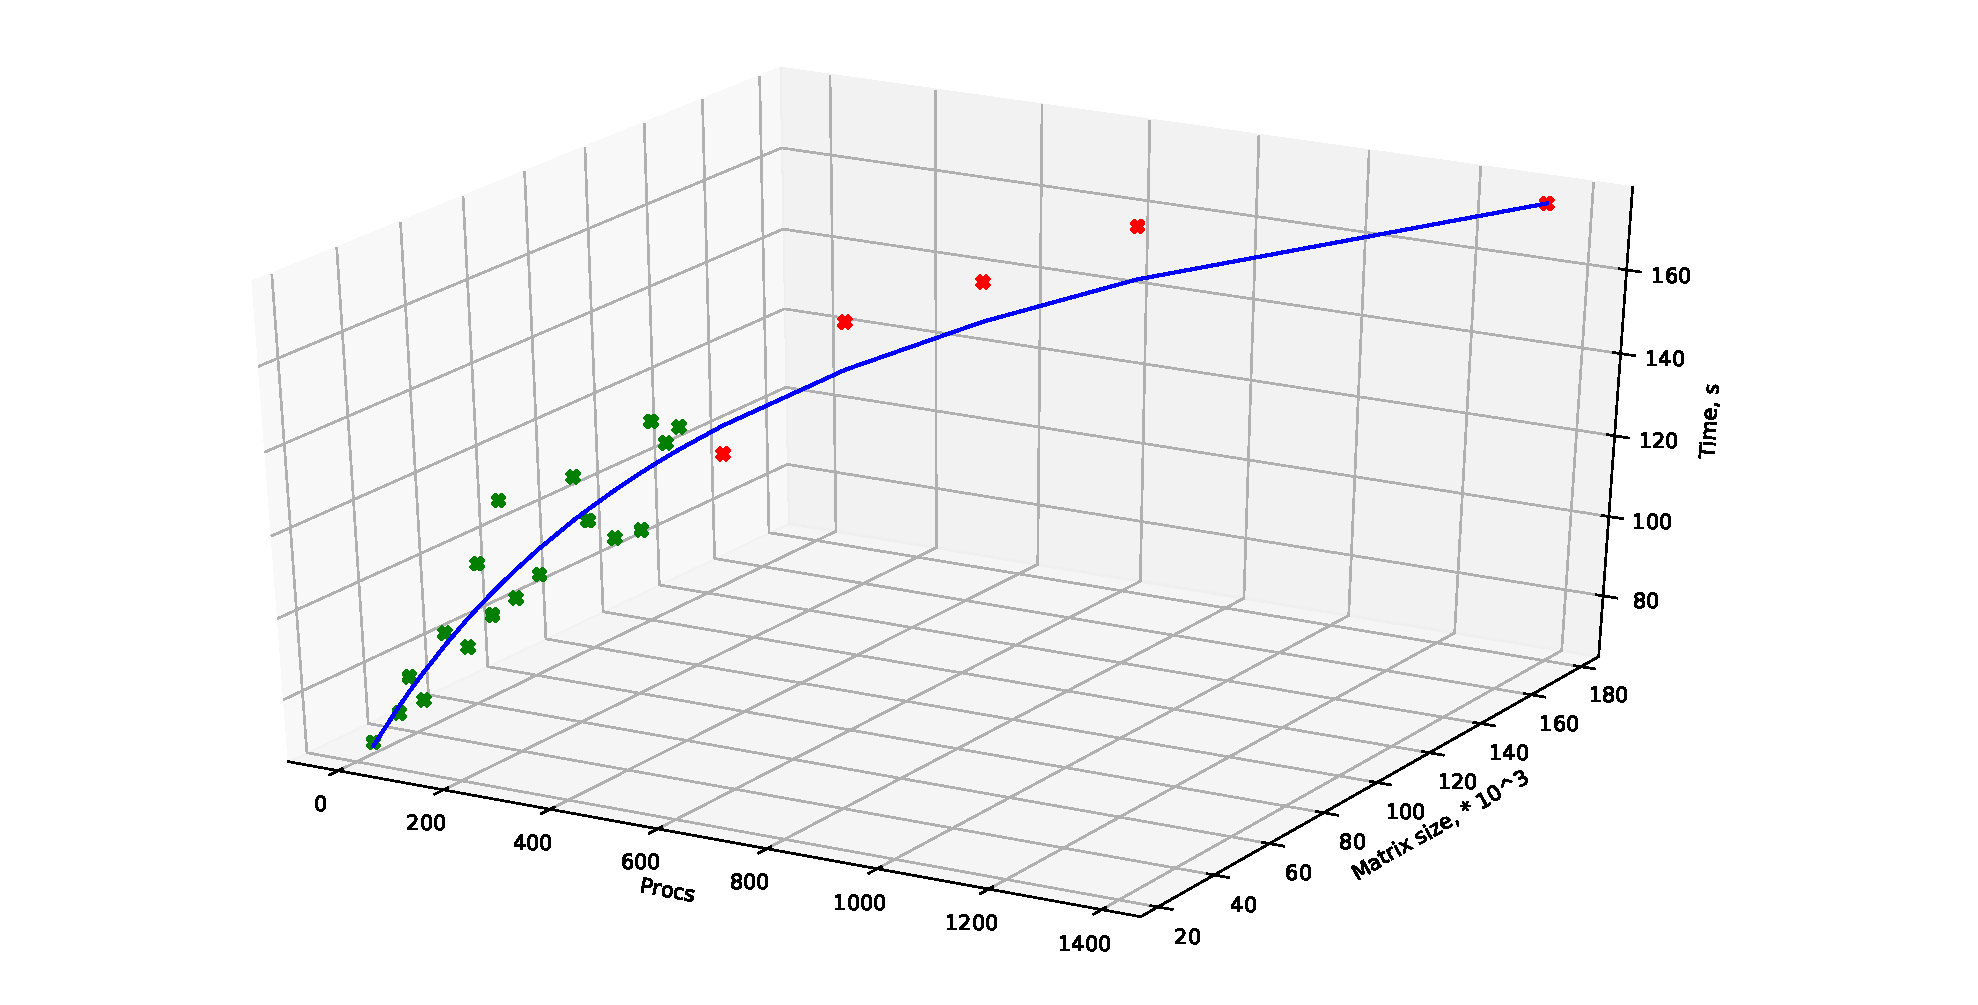
\includegraphics[width=0.9\textwidth]{./images/hpl_k3}
		\caption{Аппроксимирующая функция предсказания времени, HPL, конфигурации соответствуют константе \(C_3\)}
		\label{figure_HPL_C_3}
	\end{figure}

	Тестовые конфигурации запуска, используемые для вычислений параметров модели, и целевых конфигураций, необходимые для оценки погрешности предсказаний, приведены в таблицах \eqref{test_HPL} и \eqref{target_HPL} соответственно. Коэффициенты \(C_1, C_2, C_3\), определяющие значение отношения количества работы приходящееся на один процесс и количества используемых процессов из выражения \eqref{weak_sc} связаны соотношением: \(4 \cdot C_1 = 2 \cdot C_2 = C_3 \), то есть с увеличением на единицу номера коэффициента количество работы на один процесс увеличивается в два раза.

	Относительные ошибки для всех целевых конфигураций слабой масштабируемости HPL представлены в таблице \eqref{target_HPL}. Значения относительных ошибок предсказания времени по всем целевым конфигурациям варьируются от 0,02\% до 11,35\%, среднее значение - 4,12\%, медиана - 3,82\%, а производительности - от 0,07\% до 16,35\%, среднее значение - 5,23\%, медиана - 5,69\%. Если рассматривать более детально, как меняются относительные ошибки с увеличением числа используемых процессов и размера задачи, усредняя значение ошибок по конфигурациям с одинаковым количеством используемых процессов, 225 - 5,09\%, 400 - 7,17\%, 576 - 3,74\%, 784 - 4,43\%, 1369 - 2,95\%, то можно однозначно сказать, что увеличение конфигурации не приводит к росту значений относительных ошибок. Что говорит об отсутствии необходимости увеличивать количество тестовых конфигураций и, самое главное, способности предложенного метода предсказывать значения различных динамических характеристик на конфигурациях в 6-7 раз больших, чем самые большие тестовые. Получающуюся аппроксимирующую функцию для одной из констант можно видеть на рисунке \eqref{figure_HPL_C_3}.

	\subsection{HPCG}

	HPCG (High Performance Conjugate Gradients Benchmark) был разработан, чтобы стать альтернативной HPL метрикой оценки производительности суперкомпьютеров. HPCG сильно выделяется на фоне остальных приложений, так как и сложность последовательного алгоритма, и количество операций чтения/записи бенчмарка пропорциональны \(\mathcal{O}(N)\). В тесте преобладают нерегулярный доступ к памяти и мелкоструктурные рекурсивные вычисления, которые, как утверждают авторы бенчмарка, свойственны многих научным вычислительным приложениям \cite{HPCG}. Основное вычислительное ядро HPCG занимается решением СЛАУ с разреженной положительно определённой симметричной матрицей с помощью метода сопряжённых градиентов.

	%Для тестирования использовались следующие конфигурации запуска: тестовые - количество процессов \(q = 14 \cdot i,\ i \in \{1 \ldots 15\}\), целевые - количество процессов \(q = 14 \cdot i,\ i \in \{20, 40, 50, 70, 100\}\), размер задачи для обоих случаев задаётся как - \(q \cdot 104 \cdot 104 \cdot 104\), то есть один процесс будет обсчитывать куб со стороной \(104\).
	Тестовые и целевые конфигурации представлены в таблице \eqref{conf_HPCG}, а получившиеся относительные ошибки предсказаний в таблице \eqref{result_HPCG}. Несмотря на то что в двух случая значения относительных ошибок сильно отличаются от остальных и почти достигают 20\%, среднее имеет меньшее значение и составляет 2,674\% для предсказания времени и 8,554\% для производительности.
	\begin{table}
		\centering
		\begin{tabular}{|c|c|c|}
			\hline
			PN                          & PS                                 & Parameter \(i\)                                 \\ \hline
			\multirow{2}{*}{\(14 \cdot i\)} & \multirow{2}{*}{\(PN \cdot 104^3\)} & Тестовые: \(i \in \{1,\,\ldots,\,15\}\)         \\ \cline{3-3}
			                            &                                    & Целевые:  \(i \in \{20,\,40,\,50,\,70,\,100\}\) \\ \hline
		\end{tabular}
		\caption{Тестовые и целевые конфигурации запусков HPCG}
		\label{conf_HPCG}
	\end{table}
	\begin{table}
		\centering
		\begin{tabular}{|c|c|c|c|}
			\hline
			PN	& PS  & RE\_time & RE\_perf \\ \hline
			280 & \multirow{5}{*}{\(PN \cdot 104^3\)} & 0,02     & 0,37     \\ \cline{1-1} \cline{3-4}
			560 &     & 1,56     & 0,80     \\ \cline{1-1} \cline{3-4}
			700 &     & 1,89     & 13,07    \\ \cline{1-1} \cline{3-4}
			980	&     & 2,85     & 19,54    \\ \cline{1-1} \cline{3-4}
			1400 &    & 7,05     & 8,99     \\ \hline
		\end{tabular}
		\caption{Относительные ошибки предсказания времени и производительности HPCG}
		\label{result_HPCG}
	\end{table}

	\subsection{Алгоритмы матричного умножения}
		\subsubsection{SUMMA}
			Первый из двух рассматриваемых алгоритмов матричного умножения - SUMMA(Scalable Universal Matrix Multiply)\cite{SUMMA}. Различные реализации этого алгоритма используются такими библиотеками, как ScaLAPACK и PBLAS. Он, так же как и HPL, имеет сложность \(\mathcal{O}(N^3)\) и количество операций чтения/записи пропорционально \(\mathcal{O}(N^2)\). Тестовые и целевые конфигурации запуска приведены в таблицах \eqref{test_SUMMA} и \eqref{target_SUMMA} соответственно. Для тестирования использовалась реализация, требующая квадратной процессорной сетки, однако в общем случае это не является обязательным условием для данного алгоритма. Коротко этот алгоритм можно записать так:
			\begin{algorithm}
				\begin{algorithmic}
					\State $C_{ij} = 0$
					\For{$l = \overline{0,k - 1}$}
					\State broadcast $a_i^l$ within my row
					\State broadcast $b_l^j$ within my column
					\State $C_{ij} = C_{ij} + a_i^l \cdot {b_l^j}^T$
					\EndFor
				\label{SUMMA_algo}
				\end{algorithmic}
			\end{algorithm}

			\begin{table}
				\centering
				\begin{tabular}{|r|c|c|}
					\hline
					\textnumero & PN  & PS                     \\ \hline
					1           & 1   & 4                      \\ \hline
					2           & 4   & 6,4                    \\ \hline
					3           & 9   & 8,4                    \\ \hline
					4           & 16  & 10                     \\ \hline
					5           & 25  & 11,5                   \\ \hline
					6           & 36  & 13,2                   \\ \hline
					7           & 49  & 14,7                   \\ \hline
					8           & 64  & 16                     \\ \hline
					9           & 81  & 17,1                   \\ \hline
					10          & 100 & 18,5                   \\ \hline
					11          & 121 & 19,8                   \\ \hline
					12          & 144 & 21                     \\ \hline
					13          & 169 & 22,1                   \\ \hline
					14          & 196 & 23,1                   \\ \hline
				\end{tabular}
				\caption{Тестовые конфигурации запусков матричного умножения по алгоритму SUMMA}
				\label{test_SUMMA}
			\end{table}

		\begin{table}
			\centering
			\begin{tabular}{|r|c|c|c|}
			\hline
			\textnumero & PN   & PS   & RE\_time        \\ \hline
			1           & 225  & 25,6 & 1,95            \\ \hline
			2           & 400  & 30   & 3,94            \\ \hline
			3           & 576  & 33,6 & 3,01            \\ \hline
			4           & 784  & 37,8 & 7,59            \\ \hline
			5           & 1024 & 40   & 1,39            \\ \hline
			\end{tabular}
			\caption{Целевые конфигурации запусков матричного умножения по алгоритму SUMMA и значения относительных ошибок предсказания времени на этих конфигурациях}
			\label{target_SUMMA}
		\end{table}
		%Из-за того что исследуется предсказание масштабируемости в условиях слабой масштабируемости приложений, 
		Из-за того что строятся предсказания слабой масштабируемости приложений, то рассматриваемые конфигурации должны удовлетворят выражению \eqref{weak_sc} для некоторого значения константы. Так как известно, что данный алгоритм имеет кубическую сложность, то можно уточнить запись этого выражения: \(T_A(N)\:/\:p = const \Rightarrow p = N^3\:/\:const\). Как видно по графику зависимости количества используемых процессов от длины стороны матрицы \eqref{conf_SUMMA} конфигурации запусков выбираются строго согласно этому выражению.

		\begin{figure}
			\centering
			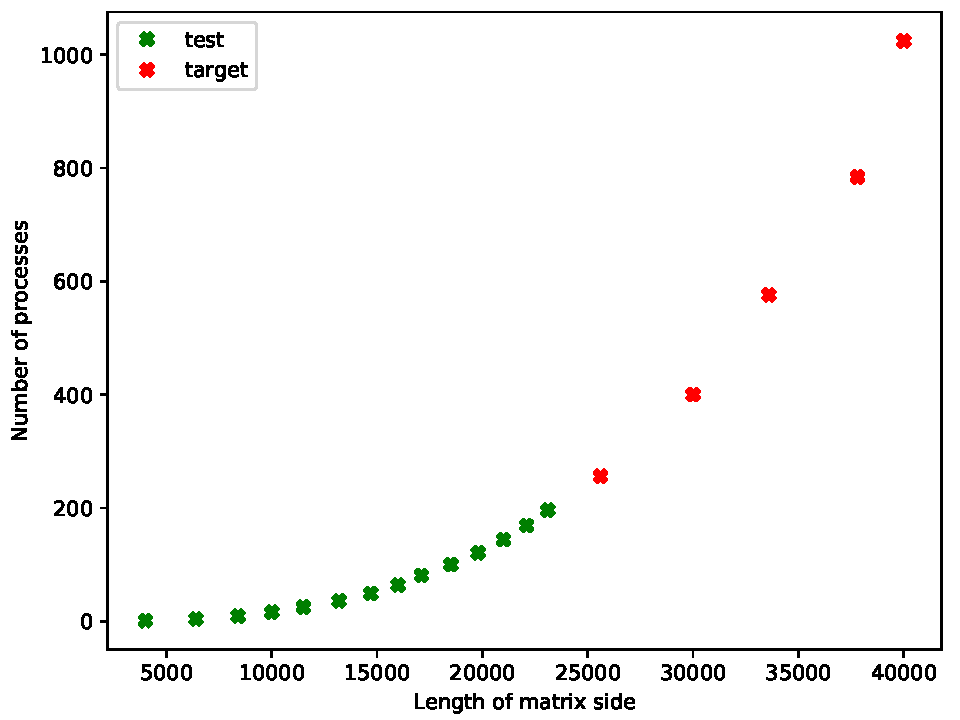
\includegraphics[width=0.5\textwidth]{./images/conf_SUMMA}
			\caption{Конфигурации запусков матричного умножения по алгоритму SUMMA}
			\label{conf_SUMMA}
		\end{figure}

		Несмотря на сложную, скачкообразную зависимость времени работы программы \eqref{graph_SUMMA} предложенному методу удаётся установить основной характер изменения времени выполнения и построить предсказание так, что среднее значение относительной ошибки равно 3,58\%, а медиана - 3,01\%, все значения относительных ошибок приведены в таблице \eqref{target_SUMMA}.

		\begin{figure}
			\centering
			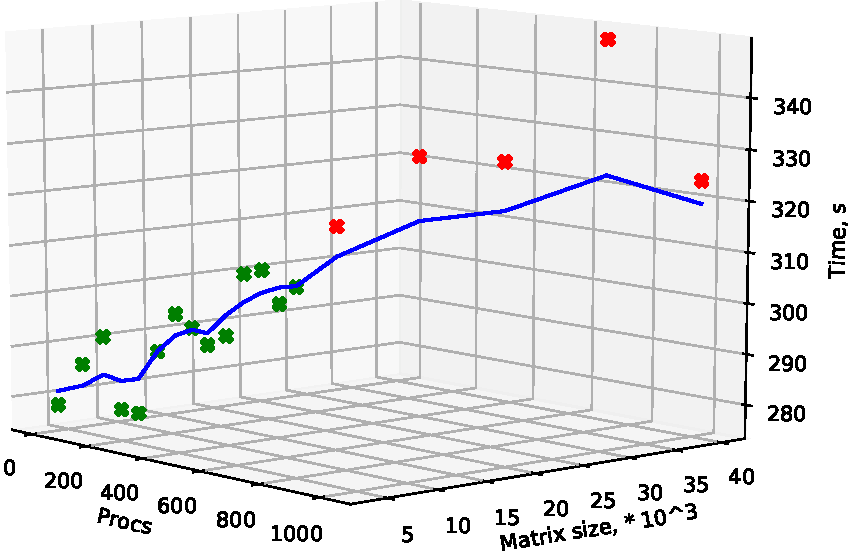
\includegraphics[width=0.9\textwidth]{./images/graph_SUMMA}
			\caption{Аппроксимирующая функция предсказания времени, SUMMA}
			\label{graph_SUMMA}
		\end{figure}
%%%%%%%%%%%%%%%%%%%%%%%%%%%%%%%%%%%%%%%%%%%%%%%%%%%%%%%%%%%%%%%%%%%%%%%%%%%%%%%%%%
		\subsubsection{DNS}
			Следующий из рассматриваемых алгоритмов матричного умножения - DNS. Для его работы необходимо, чтобы количество процессов было равно кубу некоторого натурального числа. Из этих процессов создаётся 3D решётка. Перемножаемые матрицы считываются нижним слоем решётки, делятся на блоки и рассылаются специальным образом остальным процессам. Далее происходит локальное перемножение полученных блоков матриц и пересылка получившихся значений на нижний слой, из которых там собирается результирующая матрица.

			\begin{table}
				\centering
				\begin{tabular}{|r||c|c||c|c|}
					\hline
					            & \multicolumn{2}{c||}{\(C_1\)} & \multicolumn{2}{c|}{\(C_2\)}  \\ \hline
					\textnumero & PN  & PS                      & PN  & PS                      \\ \hline
					1           & 1   & 4,5                     & 1   & 9                       \\ \hline
					2           & 8   & 9                       & 8   & 18                      \\ \hline
					3           & 27  & 13,5                    & 27  & 27                      \\ \hline
					4           & 64  & 18                      & 64  & 36                      \\ \hline
					5           & 125 & 22,5                    & 125 & 45                      \\ \hline
					6           & 216 & 27                      & 216 & 54                      \\ \hline
				\end{tabular}
				\caption{Тестовые конфигурации запусков матричного умножения по алгоритму DNS для двух различных значений констант}
				\label{test_DNS}
			\end{table}

			\begin{table}
				\centering
				\begin{tabular}{|r||c|c|c||c|c|c|}
					\hline
					            & \multicolumn{3}{|c||}{\(C_1\)} & \multicolumn{3}{c|}{\(C_2\)} \\ \hline
					\textnumero & PN   & PS   & RE\_time        & PN   & PS & RE\_time          \\ \hline
					1           & 343  & 31,5 & 6,55            & 343  & 63 & 5,66              \\ \hline
					2           & 512  & 36   & 8,42            & 512  & 72 & 6,84              \\ \hline
					3           & 729  & 40,5 & 9,35            & 729  & 81 & 7,85              \\ \hline
					4           & 1000 & 45   & 7,94            & 1000 & 90 & 1,94              \\ \hline
					5           & 1331 & 49,5 & 9,63            & 1331 & 99 & 0,19              \\ \hline
				\end{tabular}
				\caption{Целевые конфигурации запусков DNS для двух различных значений констант и значения относительных ошибок предсказания времени и производительности на этих конфигурациях}
				\label{target_DNS}
			\end{table}

			Из-за ограничения, накладываемого алгоритмом на количество используемых для запуска процессов, тестовая выборка получается достаточно маленькая, всего 6 различных конфигураций. Но, несмотря на это, среднее значение относительной ошибки составляет всего 6,43\%. Получившиеся функции-предикторы для двух рассматриваемых значений констант представлены на рисунках \eqref{graph_DNS}. С некоторого момента при увеличением размера конфигурации, независимо от рассматриваемой константы, время работы алгоритма почти прекращает расти, это говорит об его хорошей слабой масштабируемости, а то небольшое увеличение времени работы можно связать с возрастающими накладными расходами на коммуникации.

			\begin{figure}
			\begin{subfigure}{.5\textwidth}
				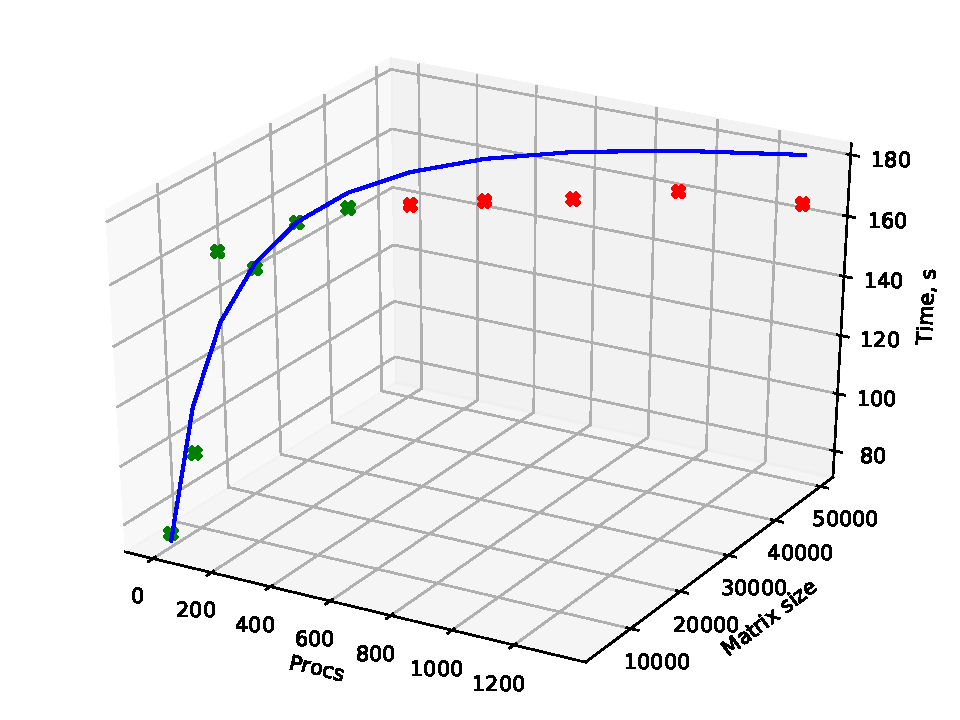
\includegraphics[width=\linewidth]{./images/graph_C_1_DNS}
				\caption{\(C_1\)}
				\label{graph_C_1_DNS}
			\end{subfigure}
			\begin{subfigure}{.5\textwidth}
				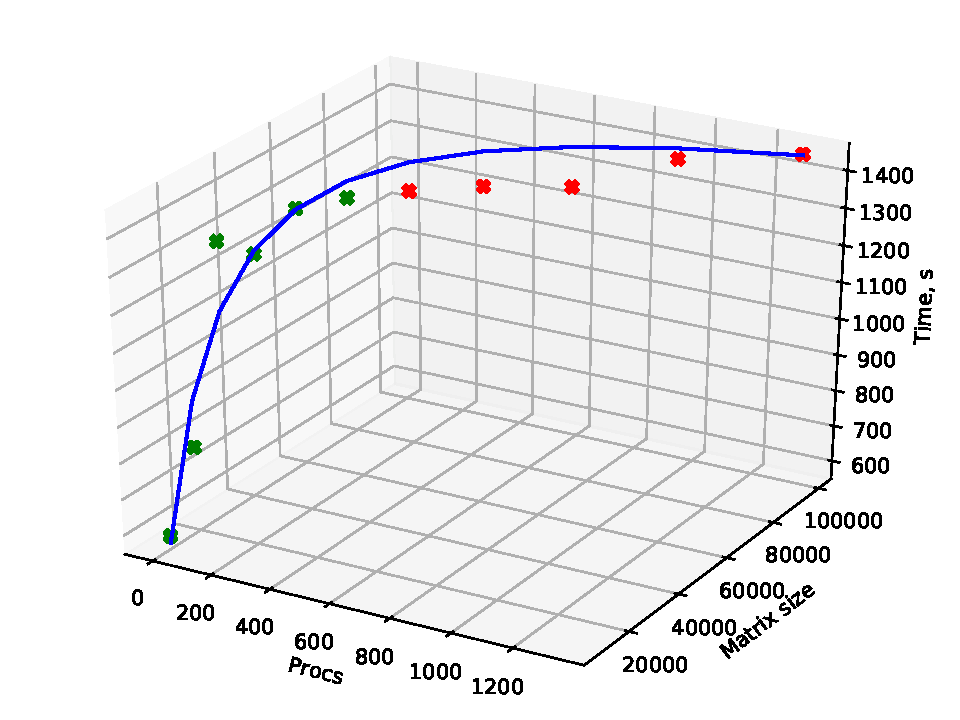
\includegraphics[width=\linewidth]{./images/graph_C_2_DNS}
				\caption{\(C_2\)}
				\label{graph_C_2_DNS}
			\end{subfigure}
			\caption{Аппроксимирующие функции предсказания времени для двух различных значений констант, DNS}
			\label{graph_DNS}
			\end{figure}

	\subsection{Graph500}
		Последнее из рассматриваемых приложений - Graph500. Это ещё одна альтернатива HPL, помимо уже ранее рассмотренного бенчмарка HPCG, по результатам работы которого также составляется рейтинг суперкомпьютеров. Однако Graph500, в отличии от HPL и HPCG, больше нагружает коммуникационную подсистему компьютера и не так сильно зависит от количества исполняемых операций над числами с плавающей запятой в секунду. Подобное поведение свойственно многим задачам из области графовой аналитики и работы с большими данными. Бенчмарк Graph500 включает в себя два графовых алгоритма: поиск в ширину (BFS) и поиск кратчайшего пути от одной вершины (SSSP). Из-за того, что в основе лежит работа с графами, то производительность измеряется не в GFlops, а в MTeps (количество пройденных дуг в секунду).

		Сложность алгоритма в случае работы с графами выражается через число его вершин и рёбер, так для Graph500 это \(\mathcal{O}(V + E)\), где \(V\)- количество вершин, а \(E\) - рёбер. Размер задачи задаётся двумя параметрами \(scale - SC\) и \(edgefactor - EF\): количество вершин графа равно \(2^{SC}\), а \(EF\) равен половине средней степени вершины графа, то есть \(EF = \frac{E}{V}\). Используя эти два параметра для вычисления сложности работы алгоритма, можно получить: \[V + E = 2^{SC} + EF \cdot 2^{SC} = 2^{SC} \cdot (1 + EF) \]

		\begin{table}
			\centering
			\begin{tabular}{|r||c|c|c||c|c|c|}
				\hline
				            & \multicolumn{3}{c||}{\(C_1\)} & \multicolumn{3}{c|}{\(C_2\)} \\ \hline
				\textnumero & PN  & SC & EF                 & PN  & SC & EF                \\ \hline
				1           & 14  & 25 & 16                 & 14  & 26 & 16                \\ \hline
				2           & 28  & 26 & 16                 & 28  & 27 & 16                \\ \hline
				3           & 42  & 26 & 25                 & 42  & 27 & 25                \\ \hline
				4           & 56  & 27 & 16                 & 56  & 28 & 16                \\ \hline
				5           & 70  & 27 & 20                 & 70  & 28 & 20                \\ \hline
				6           & 84  & 27 & 25                 & 84  & 28 & 25                \\ \hline
				7           & 98  & 27 & 29                 & 98  & 28 & 29                \\ \hline
				8           & 112 & 28 & 16                 & 112 & 29 & 16                \\ \hline
				9           & 126 & 28 & 18                 & 126 & 29 & 18                \\ \hline
				10          & 140 & 28 & 20                 & 140 & 29 & 20                \\ \hline
				11          & 154 & 28 & 22                 & 154 & 29 & 22                \\ \hline
				12          & 168 & 28 & 25                 & 168 & 29 & 25                \\ \hline
				13          & 182 & 28 & 27                 & 182 & 29 & 27                \\ \hline
				14          & 196 & 29 & 14                 & 196 & 30 & 14                \\ \hline
				15          & 210 & 29 & 15                 & 210 & 30 & 15                \\ \hline
			\end{tabular}
			\caption{Тестовые конфигурации запусков бенчмарка Graph500 для двух различных значений констант}
			\label{test_Graph500}
		\end{table}

		\begin{table}
			\centering
			\begin{tabular}{|r||c|c|c|c|c|c|c|}
				\hline
				            & \multicolumn{7}{c|}{\(C_1\)}                                                     \\ \hline
				            & PN   & SC & EF & RE\_time(BFS) & RE\_perf(BFS) & RE\_time(SSSP) & RE\_perf(SSSP) \\ \hline
				1           & 280  & 30 & 20 &          3,23 &          4,20 &           6,40 & 7,06           \\ \hline
				2           & 560  & 31 & 20 &          5,09 &          2,03 &          17,62 & 17,67          \\ \hline
				3           & 700  & 31 & 26 &         12,94 &          8,82 &           5,24 & 9,99           \\ \hline
				4           & 980  & 31 & 36 &         20,93 &         19,92 &           0,61 & 5,76           \\ \hline
				5           & 1400 & 32 & 26 &         15,59 &          8,54 &           5,29 & 12,98          \\ \hhline{|=||=|=|=|=|=|=|=|} 
				            & \multicolumn{7}{c|}{\(C_2\)}                                                     \\ \hline
				\textnumero & PN   & SC & EF & RE\_time(BFS) & RE\_perf(BFS) & RE\_time(SSSP) & RE\_perf(SSSP) \\ \hline
				1           & 280  & 29 & 20 &         12,42 &         12,03 &          16,87 & 15,05          \\ \hline
				2           & 560  & 30 & 20 &          5,08 &          7,86 &          25,16 & 21,94          \\ \hline  
				3           & 700  & 30 & 26 &          5,74 &          0,50 &          27,14 & 24,63          \\ \hline
				4           & 980  & 30 & 36 &         25,80 &         27,76 &           8,41 & 11,22          \\ \hline
				5           & 1400 & 31 & 26 &         26,45 &         24,55 &          19,61 & 21,93          \\ \hline

				              
			\end{tabular}
			\caption{Целевые конфигурации запусков бенчмарка Graph500 для двух различных значений констант и значения относительных ошибок предсказания времени и производительности на этих конфигурациях}
			\label{targer_Graph500}
		\end{table}

		Во время тестирования этого приложения становится ясно видна основная проблема определения, предсказывания слабой масштабируемости приложений: конфигурации запуска выбираются согласно отношению \eqref{weak_sc}, но не всегда возможно обеспечить строгое равенство, поэтому приходится округлять некоторые параметры запуска. Из-за этого возможны провалы или всплески показателей рассматриваемых динамических характеристик, которые сильно портят качество предсказаний. Так в случае Graph500 приходилось округлять значения \(SC\) и \(EF\), так как они могут принимать только целые значения. В связи с этим средние значения относительных ошибок предсказания времени и производительности для этого приложения составляют около 13\%.
\clearpage
%\newpage
	\section{Заключение}
	\begin{figure}
		\centering
		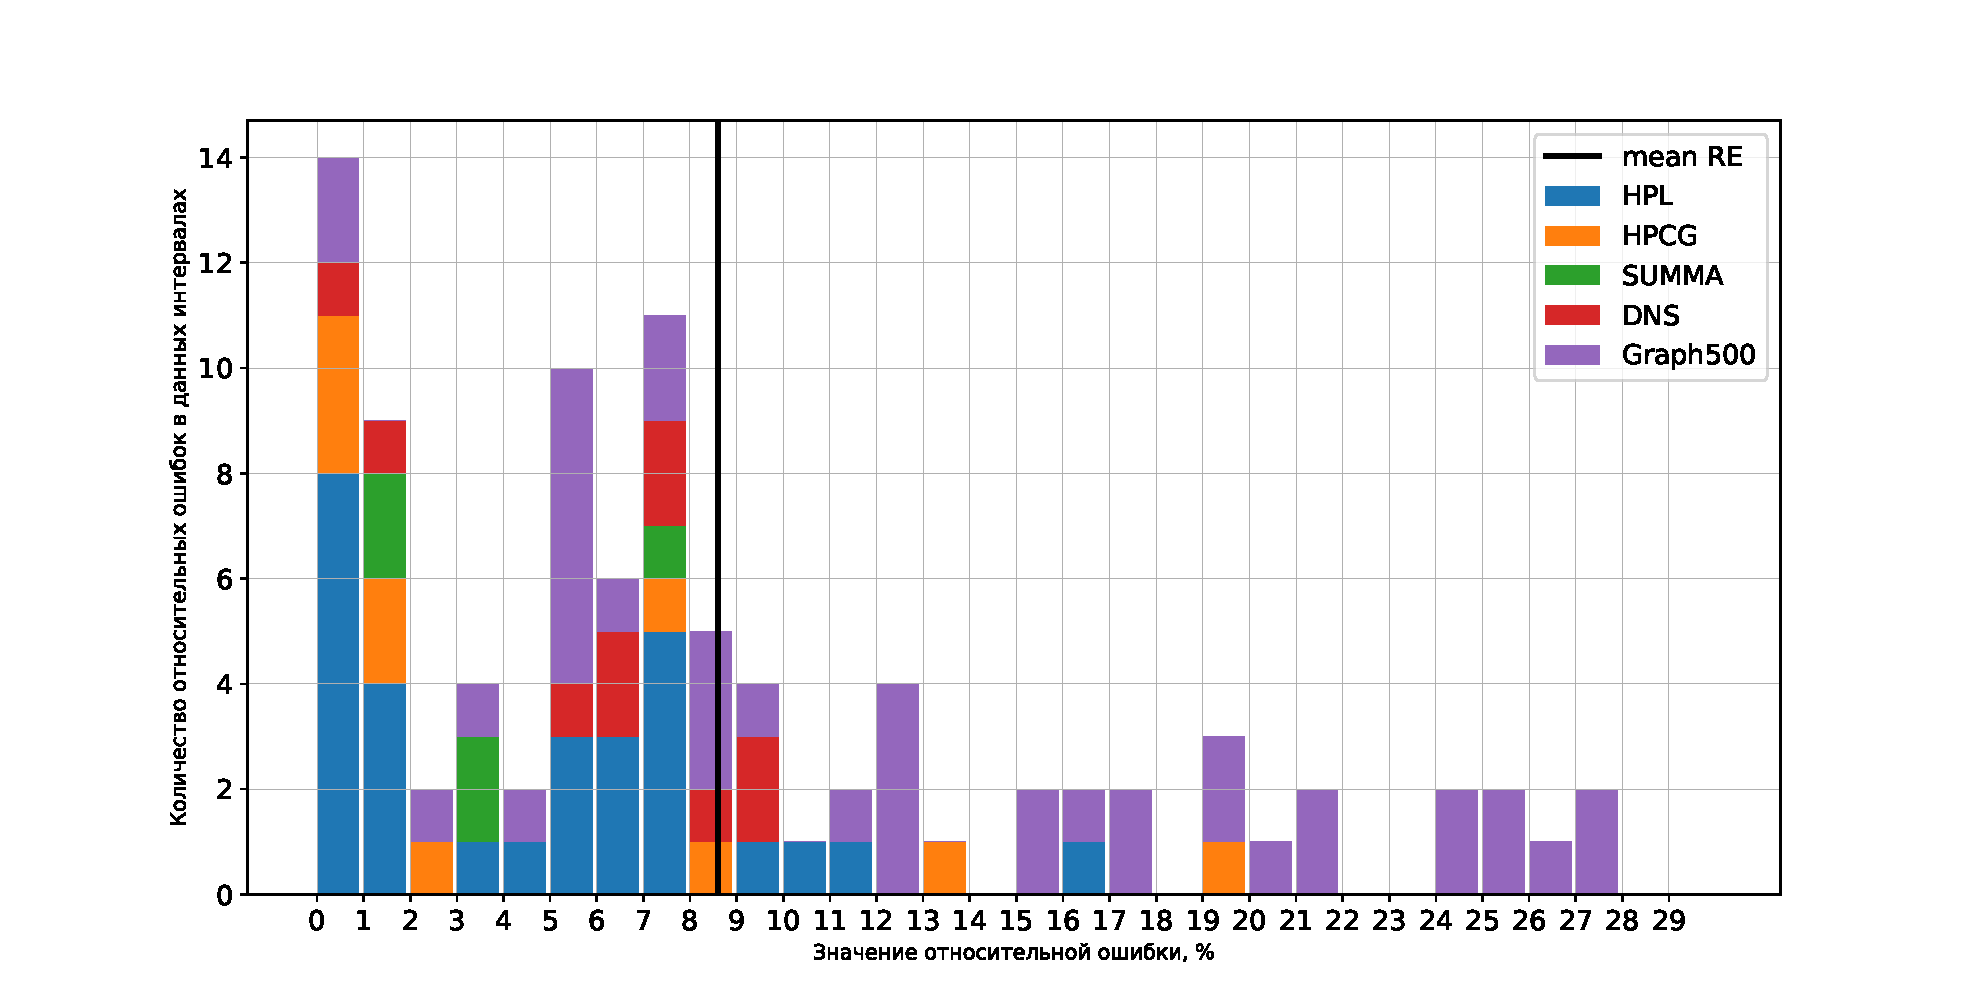
\includegraphics[width=\textwidth]{./images/RE_graph}
		\caption{Относительные ошибки предсказаний по всем рассматриваемым приложениям}
		\label{RESULT}
	\end{figure}
	В данной работе были получены следующие основные результаты:
	\begin{itemize}
		\item Разработан метод, предсказывающий слабую масштабируемость суперкомпьютерных приложений на основе экспериментальных данных со средней относительной ошибкой по всем смотренным приложениям равной 8,6\%.
		%\item Выполнена проверка применимости метода на различных приложениях, с помощью запусков приложений HPL, HPCG, матричных алгоритмов умножения SUMMA и DNS, Graph500 на суперкомпьютере "<Ломоносов-2">.
		\item Выполнена экспериментальная проверка метода с помощью запусков на суперкомпьютере "<Ломоносов-2"> на примере HPL, HPCG, алгоритмов матричного умножения (SUMMA и DNS), Graph500.
	\end{itemize}

	На основании предложенного метода удалось построить предсказания слабой масштабируемости для всех рассматриваемых приложений так, что максимальная относительная ошибка среди всех приложений и конфигураций не превышает 28\%, однако подобный значения являются единичными случаями. Средние значения относительных ошибок для различных приложений равны HPL - 4,9\%, HPCG - 5,6\%, SUMMA - 3,6\%, DNS - 6,4\%, Graph500 - 13,2\%. Так как почти треть всех предсказаний значений динамических характеристик приходится на Graph500, а на этом приложении сильнее всего отразились трудности заданием конфигураций запусков, поэтому  относительные ошибки именно на этом приложении во многом являются определяющими, при расчёте среднего значения ошибок по всем приложениям, которое составляет 8,6\%. Гистограмма с различными значениями относительных ошибок представлена на рисунке \eqref{RESULT}. Таким образом, относительные ошибки предсказания предложенного метода
	%предложенный метод предсказания даёт относительные ошибки, сравнимые 
	сравнимы с ошибками предсказания существующих подходов при сопоставимых размерах конфигураций предсказываемых запусков. Но разработанный метод отличается от них простотой построения, отсутствием необходимости собирать большой набор тестовых данных и способностью строить предсказания, не используя информацию о коде, алгоритме и системе, на которой производятся запуски, то есть он является достаточно универсальным.
	%Помимо этого, он удовлетворяет поставленным условиям универсальности.
	
\clearpage
%\newpage
	\section{Список литературы}
	\begingroup
		\renewcommand{\section}[2]{}%
		\begin{thebibliography}{}
			\bibitem{top500}
			The 54nd edition of the TOP500 list [Электронный ресурс]. – Электрон. дан. – URL: https://www.top500.org/lists/2019/11/. (дата обращения 16.03.2020).

			\bibitem{Perf_low}
			Leland, Robert \& Ang, Jim \& Barnette, Daniel \& Benner, Bob \& Goudy, Sue \& Malins, Bob \& Rajan, Mahesh \& Vaughan, Courtenay \& Black, Amalia \& Doerfler, Doug \& Domino, Stefan \& Franke, Brian \& Ganti, Anand \& Laub, Tom \& Meyer, Hal \& Scott, Ryan \& Stevenson, Joel \& Sturtevant, Judy \& Taylor, Mark. (2016). Performance, Efficiency and Effectiveness of Supercomputers.

			\bibitem{scalability_def}
			Antonov, Alexander \& Teplov, Alexey. (2016). Generalized Approach to Scalability Analysis of Parallel Applications. 291-304. 10.1007/978-3-319-49956-7\_23. 

			\bibitem{COMPLEXITY}
			Абрамов С.А. Лекции о сложности алгоритмов - М.: МЦНМО, 2012. - 245 с.

			\bibitem{scaling_types}
			Антонов, А. С., \& Теплов, А. М. (2013). Исследование масштабируемости программ с использованием инструментов анализа параллельных приложений на примере модели атмосферы Nh3d. Вестник Южно-Уральского государственного университета. Серия: Вычислительная математика и информатика, 2 (1), 5-16.

			\bibitem{log_main}
			Barnes, B. J., Reeves, J., Rountree, B., De Supinski, B., Lowenthal, D. K., \& Schulz, M. (2008). A regression-based approach to scalability prediction. In ICS'08 - Proceedings of the 2008 ACM International Conference on Supercomputing (pp. 368-377). (Proceedings of the International Conference on Supercomputing). https://doi.org/10.1145/1375527.1375580
		
			\bibitem{efficiency_prediction} 
			Rosas, C., Giménez, J., \& Labarta, J. (2014). Scalability prediction for fundamental performance factors. Supercomputing Frontiers And Innovations, 1(2), 4-19. doi:http://dx.doi.org/10.14529/jsfi140201

			\bibitem{focused_regression}
			Barnes, Brad \& Garren, Jeonifer \& Lowenthal, David \& Reeves, Jaxk \& Supinski, Bronis \& Schulz, Martin \& Rountree, Barry. (2010). Using focused regression for accurate time-constrained scaling of scientific applications. Proceedings of the 2010 IEEE International Symposium on Parallel and Distributed Processing, IPDPS 2010. 1 - 12. 10.1109/IPDPS.2010.5470431. 

			\bibitem{analytic_func}
			Alexandru Calotoiu, Torsten Hoefler, Marius Poke, and Felix Wolf. 2013. Using automated performance modeling to find scalability bugs in complex codes. In Proceedings of the International Conference on High Performance Computing, Networking, Storage and Analysis (SC ’13). Association for Computing Machinery, New York, NY, USA, Article 45, 1–12. DOI:https://doi.org/10.1145/2503210.2503277

			\bibitem{ML_SMG2000}
			Ipek E., de Supinski B.R., Schulz M., McKee S.A. (2005) An Approach to Performance Prediction for Parallel Applications. In: Cunha J.C., Medeiros P.D. (eds) Euro-Par 2005 Parallel Processing. Euro-Par 2005. Lecture Notes in Computer Science, vol 3648. Springer, Berlin, Heidelberg

			\bibitem{ML_Grid}
			Nadeem, Farrukh \& Alghazzawi, Daniyal \& Mashat, Abdulfattah \& Fakieh, Khalid \& Almalaise, Abduallah \& Hagras, Hani. (2017). Modeling and predicting execution time of scientific workflows in the Grid using radial basis function neural network. Cluster Computing. 20. 2805–2819. 10.1007/s10586-017-1018-x. 

			\bibitem{ML_PROC_KERN}
			Singh, Karan \& Curtis-Maury, Matthew \& McKee, Sally \& Blagojevic, Filip \& Nikolopoulos, Dimitrios \& Supinski, Bronis \& Schulz, Martin. (2010). Comparing Scalability Prediction Strategies on an SMP of CMPs. 6271. 143-155. 10.1007/978-3-642-15277-1\_14.

			\bibitem{simulation_FASE}
			Grobelny, Eric \& Bueno, David \& Troxel, Ian \& George, Alan \& Vetter, Jeffrey. (2007). FASE: A Framework for Scalable Performance Prediction of HPC Systems and Applications. Simulation. 83. 10.1177/0037549707084939. 

			\bibitem{representative_replay}
			Zhai, Jidong \& Chen, Wenguang \& Zheng, Weiming \& Li, Keqin. (2015). Performance Prediction for Large-Scale Parallel Applications Using Representative Replay. IEEE Transactions on Computers. 65. 1-1. 10.1109/TC.2015.2479630. 			

			\bibitem{UV_matrix}
			Shao, Qingshi \& Li, Pan \& Liu, Shijun \& Liu, Xinyan. (2017). A collaborative filtering based approach to performance prediction for parallel applications. 331-336. 10.1109/CSCWD.2017.8066716. 

			\bibitem{Kazmina_Antonov_article}
			К.П. Казьмина, А.С. Антонов. Разработка методов прогнозирования масштабируемости приложений на конфигурации суперкомпьютеров // Вестник компьютерных и информационных технологий. N 12, 2018. С. 45-56.(http://www.vkit.ru/index.php/current-issue-rus/770-045-056) DOI:10.14489/vkit.2018.12.pp.045-056

			\bibitem{Kazminf_Valkon_Antonov_article}
			Pavel Valkov, Kristina Kazmina, and Alexander Antonov. Using Empirical Data for Scalability Analysis of Parallel Applications // Communications in Computer and Information Science. Vol. 1063. 2019. Pp. 58-73. DOI:10.1007/978-3-030-28163-2\_5

			\bibitem{Lom2_stat}
			Voevodin, V., Antonov, A., Nikitenko, D., Shvets, P., Sobolev, S., Sidorov, I., Stefanov, K., Voevodin, V., \& Zhumatiy, S. (2019). Supercomputer Lomonosov-2: Large Scale, Deep Monitoring and Fine Analytics for the User Community. Supercomputing Frontiers And Innovations, 6(2), 4-11. doi:http://dx.doi.org/10.14529/jsfi190201

			\bibitem{HPCG}
			Report, S., Dongarra, J., \& Heroux, M.A. (2013). Toward a New Metric for Ranking High Performance Computing Systems.

			\bibitem{SUMMA}
			Robert A. van de Geijn and Jerrell Watts. 1995. SUMMA: Scalable Universal Matrix Multiplication Algorithm. Technical Report. University of Texas at Austin, USA.		 
		
		\end{thebibliography}
	\endgroup

\end{document}